\chapter{Implementation Broker}

\section{Request Handling}



\begin{figure}[H]
    \centering
    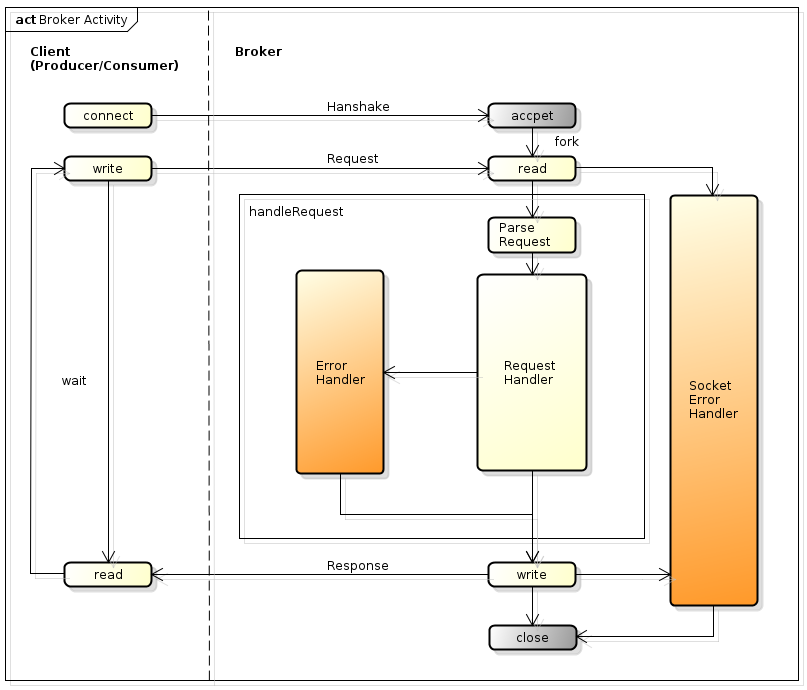
\includegraphics[width=0.7\textwidth]{images/broker-activity.png}
    \caption{Broker request handling concept}
    \label{fig:broker-activity.png}
\end{figure}

\begin{figure}[H]
    \centering
    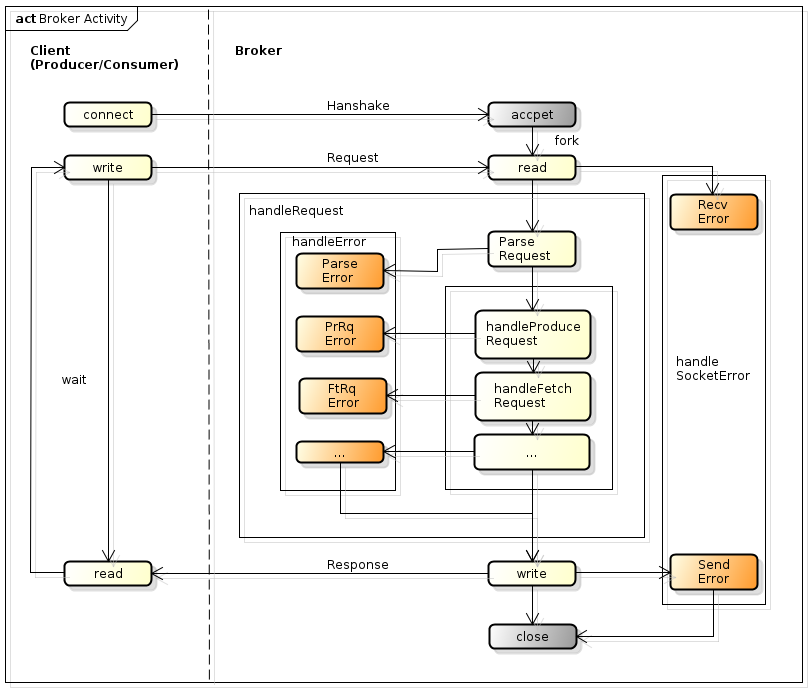
\includegraphics[width=0.7\textwidth]{images/broker-activity-detail.png}
    \caption{Broker request handling concept in detail}
    \label{fig:broker-activity-detail.png}
\end{figure}


\section{Error Handling}

\begin{figure}[H]
    \centering
    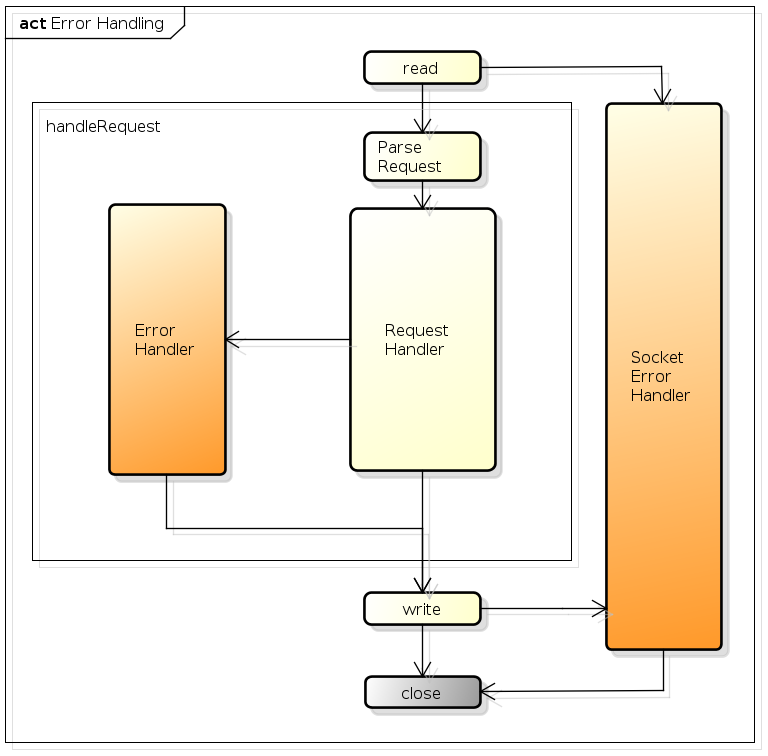
\includegraphics[width=0.7\textwidth]{images/broker-error-activity.png}
    \caption{Broker error handling concept}
    \label{fig:broker-error-activity.png}
\end{figure}


\begin{figure}[H]
    \centering
    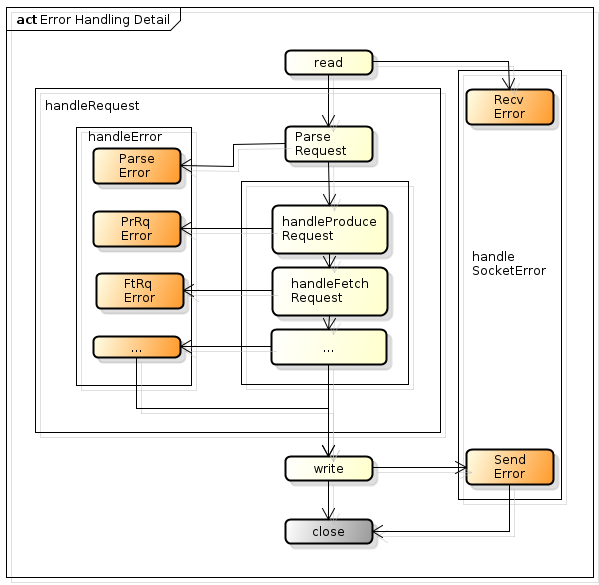
\includegraphics[width=0.7\textwidth]{images/broker-error-activity-detail.png}
    \caption{Broker handling concept in detail}
    \label{fig:broker-error-activity-detail.png}
\end{figure}


\section{Persistence}

\subsection{Storage Layout}

- for each topic a folder
- separate folders over partitions (1;2) -> topic\_0; topic\_1
- file name: offset of the first message it contains (next file: S bytes (max log size, given in configuration) from previous file)
- file format: sequence of log entries
- log entry: N (4 byte integer -> message length) followed by message (N message bytes)
- message: unique identifier (64 bit integer offset -> byte position of the start of this message in the stream of all messages ever sent to that topic on that partition)

On-disk format of a message:

offset: 8 bytes
message length : 4 bytes (value: 1+4+n) 
magic value  : 1 byte
crc            : 4 bytes
payload        : n bytes
    ?:              : 1 byte
    ?:              : 4 bytes
    message length  : 4 bytes
    message         : n bytes

\subsection{Optimization}

Next to optimizations like batching in the network layer \todo{ref to network},
we do also provide some optimizations in terms of I/O. \todo{Kafka: a
Distributed Messaging System for Log Processing}.

\subsubsection{Page Cache:}

First of all, We therefore avoid to explicitly cache messages in memory but
instead rely on the underlying file system cache. This has the benefit of
avoiding double buffering since messages are only cached in the page cache.
Thus, even if the broker process has to be restarted, the cache retains warm.

\todo{more details on modern os and page cache}

\subsubsection{Sequential I/O: }

While producers and consumers lead the broker to access
segments of files, the actual access which taking place is going to be a
sequential access rather than random. This will reduce seeking time to 1 per
partition. In fact, the broker holds a point on a given offset whereas all
messages below the pointer can be considered as already consumed and all
messages with offset greater than the provided one as unconsumed. Now since
messages are ordered this will lead to a sequential I/O with a constant seeking
time (O(1)).


\subsubsection{Internal data transfer:}

As mentioned earlier, HMB omit explicit caching but instead relies on the file system.
Keep this in mind, the actual network access for consumers can be optimized as well.
While a typical approach to sending bytes from a local file to a remote
socket involves the following steps: 
\begin{enumerate}
  \item Read data from storage (disk)
  \item Copy data from the page cache to an application buffer
  \item Copy application buffer to a kernel buffer
  \item Send kernel buffer to the socket
\end{enumerate}

With the help of the sendfile API \todo{ref} it is possible to 
transfer bytes from a file channel to a socket channel, whereas the delivery process will result in the following steps:

\begin{enumerate}
  \item Read data from storage (disk)
  \item Send data from page cache to the socket
\end{enumerate}


